\chapter{Literature Study} \label{cha:LitStudy}

\section{Introduction}
This chapter presents the literature study performed for this thesis. It consists of two parts: (i) the different path planning algorithms, on which the design of the Local Path Planner (LPP) discussed in \cref{cha:Design} is based and (ii) human-aware robot navigation, a new field in robotics that has received increasing attention from the moment that robots started working in proximity to humans. The latter part will enable the LPP to adopt a more socially compliant navigation.

\section{Path Planning Algorithms}
\Cref{sec:LPTreview} will further review the method to generate collision-free trajectories discussed in \cref{sec:ColFreeTraj} based on the following research \cite{DemeesterEtAl2012}. One of the contributions of the present thesis is to provide a more flexible set of paths, compared to those described in \cite{DemeesterEtAl2012}. Two possible approaches enabling the robot to plan a path through a challenging environment will be evaluated in \cref{sec:SLreview,sec:OMGreview} treating respectively the State Lattice path planning and an Optimal Motion Generation method. Important evaluation criteria are the local nature of the path planner, the scalability with large numbers of obstacles and the ability to provide a set of collision-free paths, which will be used to model the intention of the user.

\subsection{Local Path Template} \label{sec:LPTreview}
The LPP developed by Demeester et al. \cite{DemeesterEtAl2012} is based on the Local Path Template (LPT) method. This LPT consists of a fixed set (or template) of feasible trajectories starting from the robot's current pose (therefore local). A feasible path means that this path respects the robot's kinematic constraints.

Using a fixed set of motions brings several advantages, as the position and orientation of the robot along each path can be calculated in advance (offline) and stored in a lookup table. This lookup table contains which space the robot will take when following a particular path. The online phase consists of efficiently adjusting each path length to obtain collision-free trajectories, by using this precomputed lookup table.

However, the main disadvantage of this LPT comes with the restriction in the number and geometry of the used paths, since it is not efficient to include the full set of feasible paths that can be performed by the robot. A limit on the set must be made, thereby yielding only a (small) subset of feasible paths. However, if there are too many limitations on this set of paths, the robot will be unable to plan an otherwise kinematically feasible path which is not in the LPT. \Cref{fig:EntranceRobotLab} illustrated this problem.

The method used to create kinematically feasible paths in \cite{DemeesterEtAl2012} is to integrate achievable velocities of the wheelchair. This is commonly referred to as the forward generation method. The set of paths is obtained by integrating (maximum) allowable linear and angular velocity ($v$, $\omega$) pairs, over a certain amount of time $\Delta t$, as shown in \cref{fig:MPCircVWPair} (left). This results in a circular LPT in \cref{fig:MPCircVWPair} (right).

The main contribution of \cite{DemeesterEtAl2012} is the method used to adjust each path to obtain collision-free trajectories. This started with the observation that when paths are individually checked for collision, grid cells occupied by the robot at the start of each path are common for the majority of the paths (because all paths start from the current pose of the robot). Individual path-checking therefore results in checking several times the same grid cells, which is not efficient. Instead of building the lookup table based on each path, it can be build based on the cells occupied by the robot. In this case, cells occupied by the robot when taking each path of the LPT contain (i) which path the robot took to occupy this particular cell and (ii) its corresponding path length. The online phase will then consist of matching the occupied grid cells in the environment with cells from the lookup table. If this results in a shorter path length, then the path will be adjusted accordingly. 
\begin{figure}[!htbp]
	\centering
	\includegraphics[width=\textwidth]{MPCircVWPair.pdf}
	\doublecaption{(right) Kinematically feasible motions obtained by integrating achievable robot velocities (left)}{over a period $\Delta t = 4 s$. This results in a circular LPT, composed of 200 circular paths, including forward, backward and on the spot turning (adapted from \cite{DemeesterEtAl2012}).
	\label{fig:MPCircVWPair}}
\end{figure}

\subsection{Sate Lattice} \label{sec:SLreview}
As pointed out in \cref{sec:contribution}, a LPT exclusively based on circular curves will not always find a path in narrow passages when departing from certain start poses. A possible method of building a more flexible set of paths can be found in the research of Pivtoraiko and Kelly \cite{PivtoraikoKelly2005,PivtoraikoEtAl2009,PivtoraikoKelly2012}.

This research introduces a novel search space, the State Lattice, which represents a discrete set of states connected with feasible paths. This set of paths is called Motion Primitives (MPs) and connects nearby grids with trajectories compliant to the robot's motion constraints. \Cref{fig:SL_PP} (left) displays a possible set of MPs, which is then uniformly distributed over the whole grid to obtain the State Lattice search space, shown in \cref{fig:SL_PP} (right).

This method brings with it several advantages. Although the environment is discretized, the path connecting one state to another respects the continuity constraints of the vehicle (in the case of the wheelchair, the non-holonomic constraints). This transforms the ordinary constrained search into a minimization function, since all the connections are feasible. A certain cost should be assigned to each path of the State Lattice, for example proportional to its length, comfort, distance to obstacles.

The main focus of this research is the Global Path Planning Problem. Although this is not directly related to the local path planning, the methods described generating the set of MPs can be used to design a LPP. Pivtoraiko and Kelly describe a systematic method of generating a near-minimal set representing the MPs \cite{PivtoraikoKelly2005}. This method is based on the inverse generation method and consists of the following steps: 
\vspace{1em}
\begin{enumerate}
\item A curve geometry is chosen. For example, a polynomial curve.
\item The geometric state describing the robot are chosen (e.g. $[x,y,\theta]$) and the environment is sampled.
\item Each sampled state in the surroundings of the robot is connected using the chosen curve geometry. This is a constrained boundary value problem as only feasible paths are allowed.
\item In order to obtain a near-minimal spawning set from the origin, the notion of path decomposition has to be introduced. Each path that can be subdivided into previously calculated paths should be discarded. By doing so, an efficient set of paths is obtained resulting in faster searches.
\end{enumerate}

\begin{figure}[!tbp]
\centering
 \begin{minipage}[b]{.45\linewidth}
		\centering
		\includegraphics[width=0.85\textwidth]{SL_MP.jpg}
 \end{minipage}
 \hfill%
 \centering
 \begin{minipage}[b]{.45\linewidth}
	\centering
	 \includegraphics[width=0.85\textwidth]{SL_PP.jpg}
 \end{minipage}\\[-7pt]
 \begin{minipage}[t]{.45\linewidth}
 \end{minipage}
 \hfill
 \begin{minipage}[t]{.45\linewidth}
 \end{minipage}
	 \doublecaption{State Lattice search space based on a set of feasible motions.}{(left) A set of MPs is obtained by connecting end poses (states) with feasible trajectories from the origin. (right) By repeating the MPs uniformly, an efficient search space is obtained called the State Lattice, consisting only of feasible connections between states. An optimal path between a start- and end pose is found by minimizing an objective function represented by the cost to travel from one state to another (adapted from \cite{PivtoraikoEtAl2009}).\label{fig:SL_PP}}
\end{figure}

\newpage

\subsection{Optimal Motion Generation} \label{sec:OMGreview}
The MECO (Motion Estimation, Control and Optimization) research group of the Department of Mechanical Engineering of the KU Leuven has developed a freely available toolbox \cite{MercyVanParys2017} for Optimal Motion Generation. Based on the following research \cite{MercyEtAl2016}, \cite{VanParysPipeleers2016}, \cite{VanParysPipeleers2017}, this toolbox uses spline based motion planning for path planning in an environment including both static and dynamic obstacles. 

Three main challenges arise when trying to find an optimal (in terms of speed, safety and energy consumption) trajectory between a start and end position while respecting the system's constraints and avoiding obstacles \cite{MercyEtAl2016}.
(i) The geometric constraints, obstacle avoidance, kinematic constraints and actuator limits translate into hard non-convex problems. Optimal solutions are not guaranteed because of the local minima and are difficult to find, certainly in real-time. 
(ii) The constraints mentioned in (i) should be respected during the whole motion, not only at discrete time intervals. 
(iii) The environment in which the system operates has a degree of uncertainty. The obtained motion trajectory should be continuously updated using the most recent information on that environment.

These three challenges are addressed by using B-spline parameterization, which guarantees that the constraints are respected at all times \cite{VanLoockEtAl2015}. Time-varying separating hyperplanes are used to enforce collision-free paths along the trajectory as shown in \cref{fig:SeparatingHyperPlane}. This is calculated in real-time and continuously updated to cope with the uncertainty in the perceived environment. A robust path planning tool is obtained by using an appropriate motion model for the obstacles and by updating the planned motion to cope with unknown obstacles. Several scenarios are provided in \cref{fig:OMG_Example} as illustration.

\begin{figure}[!htbp]
	\centering
	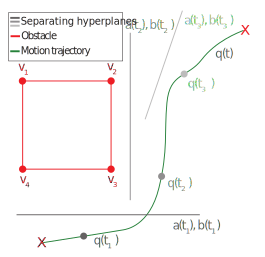
\includegraphics[width=0.5\textwidth]{SeparatingHyperPlane.pdf}
	\doublecaption{Obstacle avoidance obtained by using time-varying separating hyperplanes.}{At each discrete time instant, a hyperplane (a straight line in this 2D example) should be drawn to separate the obstacle from the robot. $a(t)$ and $b(t)$ are the 2 parameters needed to define the hyperplane. $q(t) = [x(t), y(t)]^T$ represents the state of the robot and therefore the motion trajectory to be followed (from \cite{MercyEtAl2016}).\label{fig:SeparatingHyperPlane}}
\end{figure}

\begin{figure}[!htbp]
	\centering
	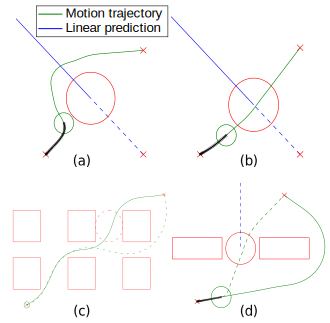
\includegraphics[width=0.59\textwidth]{OMG_Example.pdf}
	\doublecaption{Different examples for Optimal Motion Generation.}{In (a), an inappropriate motion model is assigned to the moving circle (object is assumed static even though it is moving along the blue line), leading to a possible collision. (b) Uses a correct obstacle motion model yielding a safe trajectory. In (c) an unexpected additional obstacle (dashed lines) is encountered, requiring a different path to the destination to be calculated. In (d), the circular obstacle starts moving, enabling the planner to find a shorter path through the narrow doorway (from \cite{MercyEtAl2016}). \label{fig:OMG_Example}}
\end{figure}

Although this method appears promising to obtain a flexible path, some important problems remain if it were implemented with the current Wheelchair Navigation Assistance scheme, as reviewed in \cref{sec:CurrentResearch}.
\vspace{1em}
\begin{itemize}
\item The current algorithm used to estimate the wheelchair driver's intention needs a whole set of feasible paths, which will result in solving $n$ times a slightly different constrained optimization function. This will result in a slow calculation of the set of feasible trajectories, which is not acceptable in this situation.
\item It is not clear whether (i) this method scales well in a real-world environment with a lot of obstacles and (ii) how the method would cope with non-convex obstacles and robot geometry.
\item By continuously solving a constrained optimization online, the main advantage of having a fixed set of local paths is lost. 
\end{itemize}
\vspace{1em}

The toolbox developed by MECO is particularly well suited for the use in autonomous systems. The method is, however, less adapted to situations where the intention of the user is unknown and must be continuously estimated (like a sAMR). The current intention estimation method needs a whole set of trajectories to work and therefore requires solving several times an optimization function, which necessitates too much time.

\newpage

\section{Human-Aware Robot Navigation}
This section discusses human-aware robot navigation. \Cref{sec:HARNrev} is mostly based on the survey by Kruse et al. \cite{KruseEtAl2013} and articles reviewed as part of their survey. \Cref{sec:HRCrev} focuses on a novel solution based on human-robot cooperation, to solve the ``Freezing Robot Problem'' (FRP), which happens when the robot's surroundings exceed a level of dynamic complexity. This research has been performed by Trautman et al. \cite{TrautmanEtAl2015}, which is the first publication providing a large empirical study to validate their study on navigation techniques in populated environments. This topic is especially relevant for wheelchair navigation in dense human crowds, as solving the FRP will contribute towards safer and more efficient navigation.

\subsection{Rationale and Research Areas} \label{sec:HARNrev}
Path planning for autonomous robots has become a mature field in robotics. Even in environments outside factories or other controlled areas, autonomous systems have proven their robustness in navigation among humans. For example, the research performed by Prassler et al. \cite{PrasslerEtAl1999} in 1999 introduced an autonomous wheelchair navigating in a railway station during rush hour, without any reported collision with pedestrians.

Although not colliding with the environment is an essential skill of any autonomous system, this is certainly not the only important aspect to obtain systems which are accepted and work well alongside humans. A new field focusing on increased awareness by robots of humans in the environment has emerged over the last few years. Human-aware robot navigation combines the field of human-robot interaction and robot motion planning to obtain a robotic system that is not only reliable but also accepted by humans in their new work environments. Whilst this human-robot interaction was not discussed in \cite{PrasslerEtAl1999} as per above, one can only imagine that the obstacle avoidance of the wheelchair consisted of fast and unpredictable evasive maneuvers, or just standing still if no collision-free path was found, both of which can cause confusion for the surrounding crowd. This is not a desirable interaction, as this way of navigating does not take into account that the surrounding crowd can react to and even cooperate with the wheelchair.

According to the research of Kruse et al \cite{KruseEtAl2013}, human-aware robot navigation can be divided in three different fields of research: comfort, naturalness and sociability.

\textbf{Comfort: }
The robot should not cause any stress or annoyance to the humans interacting with it. It should therefore not only be safe but be understood as safe by the interacting humans. The study of proxemics is therefore essential to avoid discomfort. Hall \cite{Hall1966} has conducted an elaborate research on the different comfort zones around a standing person during human-human interaction. Each of the zones are reserved for a different social interaction defined by a distance to the person (intimate, personal, social and public distance). Although these different comfort zones are also used as guidelines for human-robot interaction, it is important to note that the influence of dynamics (moving persons or robots) on these zones has not been properly studied so far. These dynamic factors include among others whether the person is sitting or standing and the shape and size of the approaching robot.

\textbf{Naturalness: }
The robot's behavior on a ``low level'' should reflect human motion patterns. A first step is to mimic human mobility by obtaining a jerkless motion, since humans try to be as energy efficient as possible in their movements \cite{ArechavaletaEtAl2008}. Also, a robot action should be legible (readable), meaning that the interacting humans can interpret the robot's behavior and judge its current and future actions. When a robot has legible actions, it becomes possible to have some form of cooperation between the robot and the human to facilitate the completion of each one's individual task. This is particularly important when planning a motion in a crowded environment. If the robot doesn't anticipate human cooperation, it will be unable to plan a path through or following the crowd and will try to evade it.

\textbf{Sociability: }
The robot's behavior on a ``high level'' should be similar to that of a human. This includes cultural conventions (e.g. lane side right/left) and other social protocols. E.g. skipping people in a lane and going back into the lane could be done without discomforting humans and come across as natural, but is certainly not an acceptable social behavior. Social behavior can also help in the navigation in a crowded environment, since this can be used to predict in some way the motion of pedestrians, which typically form virtual lanes when walking in close formation \cite{Helbing1991}.

\subsection{Human-Robot Cooperation} \label{sec:HRCrev}
From the moment dynamic objects (e.g. humans) in the immediate surroundings of the robot perform movements that are too complex for the path planner; the latter is unable to make suitable decisions and the robot suddenly stops or performs dangerous or unpredictable evasive maneuvers. This phenomenon is commonly referred to as the FRP. As can be seen in \cref{fig:FRP} (left), the robot (black star) tries to predict the future location of the surrounding agents (humans, red ellipses). As there is no precise motion model of the agent's movements, the uncertainty of the agent's location becomes too large for the robot to make an informed decision. It is unable to plan a path to the goal (green star).

A naive solution would be to try to achieve a good individual motion model prediction for the agents. This would work, if the crowd is sparse (\cref{fig:FRP}, right). However, from the moment the crowd is more numerous or adopts a complex formation (e.g. shoulder to shoulder walking) each independent navigation planner is bound to fail as shown in \cref{fig:HuRoCo}. Even if the predictive motion covariance is extremely low, the robot will try to pass around this formation.

\begin{figure}[!htbp]
	\centering
	\includegraphics[width=0.49\textwidth]{FRP1.jpg}
	\hfill
	\includegraphics[width=0.49\textwidth]{FRP2.jpg}
	\doublecaption{The FRP}{(left) is caused by an uncertainty explosion of the agents future location (red ellipses) due to an inaccurate motion model. The robot (black star) is therefore unable to make a decision on how to navigate through this crowd to reach the goal (green star) and stops moving. (right) When having a very low covariance on the motion prediction of each individual agent, the robot is able to plan a path when the crowd is sparse enough (from \cite{TrautmanEtAl2015}).\label{fig:FRP}}
\end{figure}

The authors of \cite{TrautmanEtAl2015} found a possible solution by inspiring themselves on how humans themselves manage to navigate in large dense crowds. Humans typically solve this problem by forming a ``joint collision avoidance'' scheme, where every agent adapts his path according to the surroundings to allow passage for everyone. Therefore, the authors redefined the ill-formulated independent path planner to explicitly expect cooperation from humans. Their method, named Interactive Gaussian Process, models the robot as part of the human crowd, and expects that all agents adapt their path so that everyone can reach their destination.

\begin{figure}[!htbp]
	\centering
	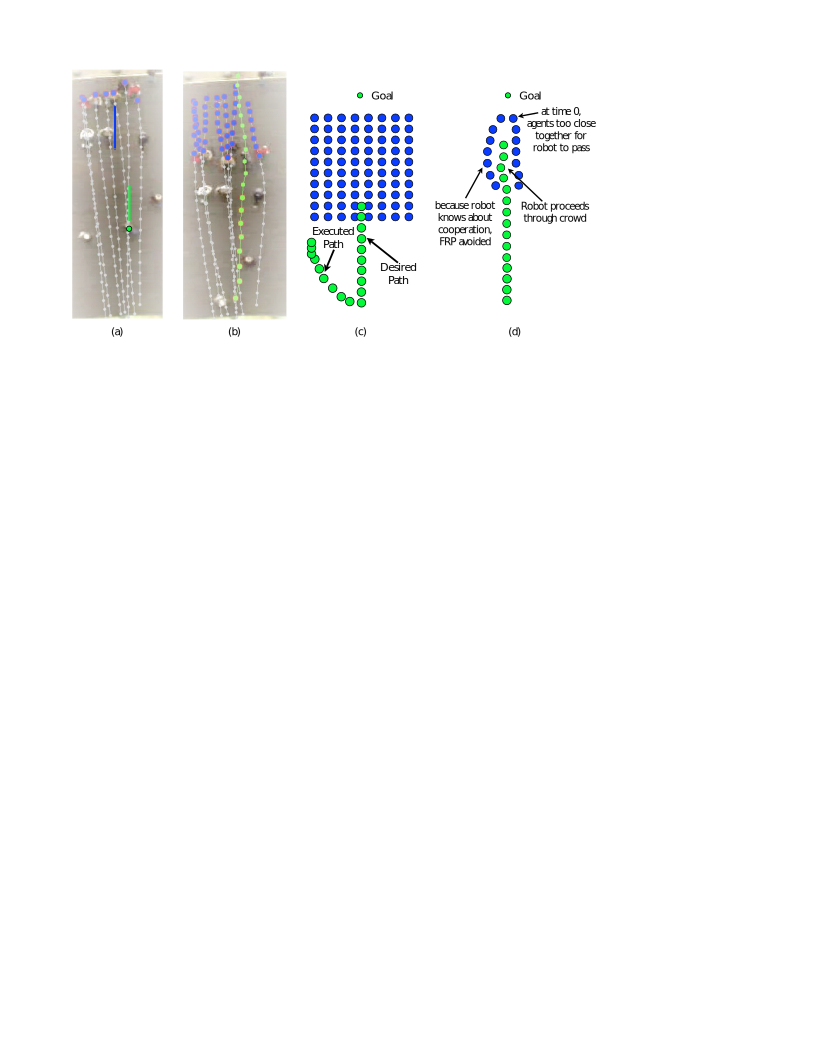
\includegraphics[width=1\textwidth]{HuRoCo.png}
	\doublecaption{Shoulder to shoulder formation makes the robot unable to plan an efficient path when relying on an independent planner.}{(a)-(b) Shows an example of joint collision avoidance. In (a), the group of people (blue dots) has not yet seen the person going up (green dot), their trajectory projection (grey line) is very narrow. In (b), everyone has adjusted their trajectory to create space. (c) Even with perfect motion prediction, the independent motion planner will not capture the cooperation between the robot (green) and the people (blue) and therefore perform an evasive maneuver even though the group of pedestrians is willing to make passage for the incoming robot. (d) Modelling this cooperation avoids the FRP (adapted from \cite{TrautmanEtAl2015}).\label{fig:HuRoCo}}
\end{figure}

\section{Conclusion} \label{sec:ConclusionReview}
The LPP to be designed in \cref{cha:Design} will contribute to the work described in \cref{sec:LPTreview} by using methods elaborated by Pivtoraiko and Kelly (\cref{sec:SLreview}). Important aspects of human-aware navigation will be considered, to obtain a LPP which inherently takes into account important aspects (comfort, naturalness and sociability) of navigation among humans. The integration of the human-robot cooperation model elaborated in \cite{TrautmanEtAl2015} in the LPP is also critical as this will enable to achieve a more robust navigation scheme when navigating in dense crowds and will therefore solve the FRP typically occurring in this type of environment. Whilst mathematical models of this cooperation model are further elaborated in \cref{sec:Cooperation}, they have not been formally implemented within the framework of this current thesis.